\documentclass[a4paper,12pt]{article}
\usepackage[UTF8]{ctex}
\usepackage{graphicx}
\usepackage{amsmath}

\begin{document}
	
\title{My First Document}
\author{My Name}
\date{\today}
\maketitle
\pagenumbering{roman}
\tableofcontents
\newpage

	
\section{Introduction}
This is the introduction

\section{Methods}

\subsection{Stage 1}
\label{sec1}
The first part of the methods.  


\subsection{Stage 2}
The second part of the methods\\ % 换行


\section{Result}
Here is my result.Referring to section \ref{sec1} on page \pageref{sec1}
	
\section{List}
\begin{enumerate}
	\item First thing
	\item Second thing
	\begin{itemize}
		\item A sub-thing
		\item Another sub-thing
	\end{itemize}
	\item Third thing
\end{enumerate}

\section{Tabular}

\begin{tabular}{|l|r|r|}
	Item & Quantity & Price(\$) \\
	\hline
	Nails & 500 & 0.34 \\
	Wooden boards & 100 & 4.00 \\
	Bricks & 240 & 11.50 \\
\end{tabular}
	
	
\begin{tabular}{c|ccc}
	& Year &  & \\
	\cline{2-4}
	City & 2006 & 2007 & 2008 \\
	\hline
	London & 45789 & 46551 & 51298 \\
	Berlin & 34549 & 32543 & 29870 \\
	Paris & 49835 & 51009 & 51970 \\
\end{tabular}


\begin{figure}[h]
	\centering
	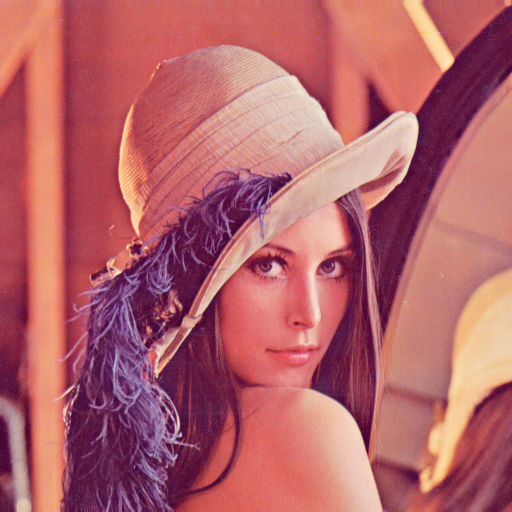
\includegraphics[width=1\textwidth]{lena}
	\caption{Here is my image}
	\label{image-myimage}
\end{figure}


\section{Formula}

\[3 + 3 = 6\]
\[n^2\]
\[2_a\]
\[\frac{a}{3}\]
\[\frac{y}{\frac{3}{x} + b}\]
\[\sqrt[5]{y^2}\]
\[\sum_{x=1}^5 y^z\]
\[\int_a^b f(x)\]


\begin{align}
	e = mc^2 \\
	\pi = \frac{c}{d} \\
	\frac{d}{dx}e^x = e^x \\
	\frac{d}{dx}\int_0^\infty f(s)ds = f(x) \\
	f(x) = \sum_i0^\infty \frac{f^(i)(0)}{i!} x^i \\
	x = \sqrt{\frac{x_i}{z} y}
\end{align}


\end{document}
